% Prelim, Chapter 2
% by Rachel Slaybaugh

\chapter{Upscattering and Energy Decomposition}
\label{sec:Chp2}
The first piece that was added to Denovo to accelerate the code was the multigroup Krylov solver. The second two methods rely on the energy decomposition and improved convergence added by this solver, so its functionality is essential to all subsequent work. The multigroup Krylov solver works very well and is a key element in accomplishing the goals of this work. 

First, the limitations of the existing parallel decomposition in Denovo for solving challenging problems are explained. Next, the background section discusses scattering and some solver basics, including an overview of Krylov subspace methods and why they are of interest for solving the transport equation. The next section focuses on existing methods used to solve the fixed source transport equation and relevant past work. Finally, a description of the new method and associated results are presented.

\section{Denovo and Parallelism}
\label{sec:DenAndPar}
To be able to solve the very large problems of interest on machines the size of Jaguar, codes that have good scaling properties are required. Recall that Denovo is parallelized in space and angle. This is done with the Koch-Baker-Alcouffe (KBA)~\cite{Baker1998} parallel sweep algorithm on a Cartesian grid. The KBA algorithm governs Denovo's parallel behavior, including how many cores it can efficiently use. To see why parallelization in energy is needed, the KBA algorithm is explained and some illustrative Denovo calculations are presented.

Angular parallelization is done by algorithmically ``stacking'' the calculation directions (ordinates) into a ``pipe'' and following more than one at a time. The transport sweeps begin with the first direction in the first quadrant and spatially move through the geometry along that ordinate in a hyper-plane fashion. Denovo uses a pipelining approach in direction such that the next angle set in an octant is started as soon as the current sweep reaches the opposite end of the geometry. The quadrants are ordered such that the next quadrant begins at the earliest possible time \cite{Evans2009d}. 

The spatial decomposition is done by assigning groups of spatial cells to different cores. A given problem will contain $(I, J, K)$ total global \emph{cells}. These are decomposed in $x$ and $y$ across $P_{I}$ cores in the $x$-direction and $P_{J}$ cores in the $y$-direction for a total of $P_{I} \times P_{J}$ cores. Each core gets a \emph{domain} that is made up of $(I_{b}, J_{b}, K)$ cells. Here $I_{b} = I/P_{I}$ and $J_{b} = J/P_{J}$. Each domain is algorithmically split into $B_{K}$ computational blocks in the $z$-direction (but not split in memory, all $K$ cells in the $z$-direction are on all cores). This creates \emph{computational blocks} of size $(I_{b}, J_{b}, K_{b})$, where $K_{b} = K/B_{K}$. The computational blocks are used in the angular pipelining process. Specifying the number of cores dictates $P_{I}$ and $P_{J}$, while the user is free to select $B_{K}$. See Figure \ref{fig:BlockDecomp} for an example of a decomposition.

\begin{figure}[!ht]	
  \begin{center}
    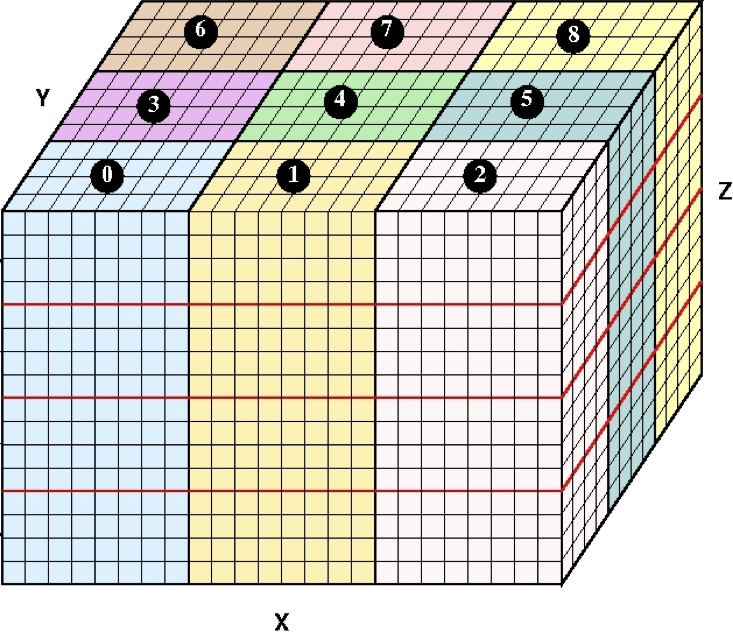
\includegraphics [width=0.6\textwidth, height=0.4\textheight ] {BlockDecompCropped}
  \end{center}
  \caption{Decomposition of 3-D mesh for KBA. In this example, the grid is decomposed on nine processors. The red lines indicated computational blocks in the $z$-direction. Each processor has $I_{b} \times J_{b} \times K$ cells, and each computational block has size $I_{b} \times J_{b} \times K_{b}$.}
  \label{fig:BlockDecomp}
\end{figure}

The decomposition parameters can be used to express the theoretical efficiency of the algorithm, which is the ratio of useful computations to total computations \cite{Evans2009d}, \cite{Baker1998}:
%
\begin{equation}
  \epsilon_{max} = \frac{2MB_{K}}{2MB_{K} + P_{I} + P_{J} - 2} \:, 
  \label{eq:efficiency}
\end{equation}
%
where $M$ is the number of directions in an octant. Note that for a set $M$, $P_{I}$, and $P_{J}$, the theoretical efficiency will be much higher when there is a larger $B_{K}$, meaning more computational blocks. Having more computational blocks creates blocks that are smaller, so work can be passed to subsequent blocks more rapidly and thus more work should be able to be done at once. The effect of $B_{K}$ on theoretical performance can be seen in the strong scaling study shown below. See \cite{Baker1998} for more details about the KBA algorithm.

The quality of parallelization can be measured in several ways. Strong scaling measures how the time to solution varies with the number of cores for a fixed problem size. Weak scaling measures how the time to solution varies with the addition of more cores when the problem size per core is fixed \cite{Bush2010}. Another factor is the total number of cores that can be used efficiently. 

A weak scaling study was performed by Evans et.\ al.\ on the Jaguar machine using a full-facility pressurized water reactor model, called the PWR900. The base-case time was generated using 4,096 cores with 103,716,288 unknowns, or $\sim$25,300 unknowns/core. When 40,000 cores and 1,046,879,390 unknowns ($\sim$26,200 unknowns/core or about a 3\% increase in problem size/core) were used, there was a 43\% increase in time to solution. The time increase for perfect weak scaling would have been about 3\%. The significant increase in time can be attributed to load-balancing latencies associated with KBA \cite{Evans2009d}. Adding parallelization over energy might improve the weak scaling properties of Denovo by making up for some of the latencies that come from KBA.

A strong scaling study was done as a part of this work that used the Jaguar machine to investigate the effect of $B_{K}$ on efficiency. A variant of the Kobayashi benchmark problem 1 \cite{Kobayashi2000}, which can be seen in Figure~\ref{fig:Kob1}, was used where the total cross sections were changed as indicated in Table~\ref{tab:Kob1xsecs}. The scattering cross sections were simply set to 0.5 $\times \Macro$ in both the original and modified case. The calculation was done with $S_{16}$, $P_{0}$, step characteristic spatial differencing, and a 0.25 cm spatial resolution, giving a 400 $\times$ 400 $\times$ 400 mesh. The number of cores was varied between 12 and 3,600. 

\begin{figure}[!ht]	
  \begin{center}
    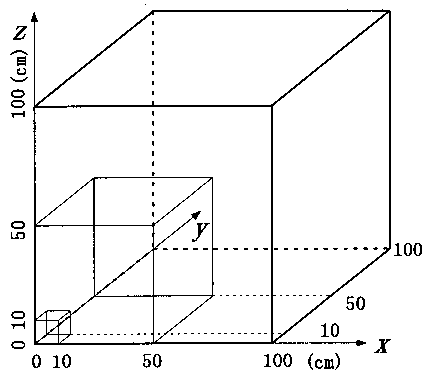
\includegraphics [width=0.4\textwidth, height=0.3\textheight ] {Kobayashi1} \\
    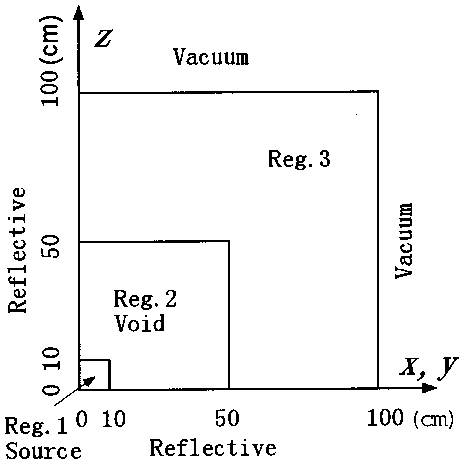
\includegraphics [width=0.4\textwidth, height=0.3\textheight ] {Kobayashi1Front}
  \end{center}
  \caption{Kobayashi Benchmark Problem 1, Two Views}
  \label{fig:Kob1}
\end{figure}

\begin{table}[h]
  \caption{Kobayashi Benchmark Problem 1, Cross Sections and Sources}
  \centering
  \begin{tabular}{|c|c|c|c|}
    \hline
    Region & S & Original $\Macro$ & Modified $\Macro$ \\
    (\#) & ($n$ cm$^{-3}$s$^{-1}$) & (cm$^{-1}$) & (cm$^{-1}$) \\
    \hline
    1 & 1 & 0.1 & 1 \\
    2 & 0 & 10$^{-4}$ & 10$^{-3}$ \\
    3 & 0 & 0.1 & 1 \\
    \hline
  \end{tabular}
  \label{tab:Kob1xsecs}
\end{table}

One set of calculations was done using $B_{K}$ = 40, or relatively many blocks, and one set using $B_{K}$ = 5, or relatively few blocks. Recall from Equation \eqref{eq:efficiency} that more computational blocks should give higher efficiency. The theoretical and actual results are plotted in Figure~\ref{fig:JagBlockStudy} as computational efficiency as a function of the number of cores used. The actual efficiency is $\frac{N_{ref}t_{ref}}{Nt}$. Here $N_{ref}$ and $t_{ref}$ are the reference number of cores and solve time, respectively, and $N$ and $t$ are for the calculation in question.  The theoretical efficiency was calculated using Equation \eqref{eq:efficiency}.

\begin{figure}[!h]
  \begin{center}
    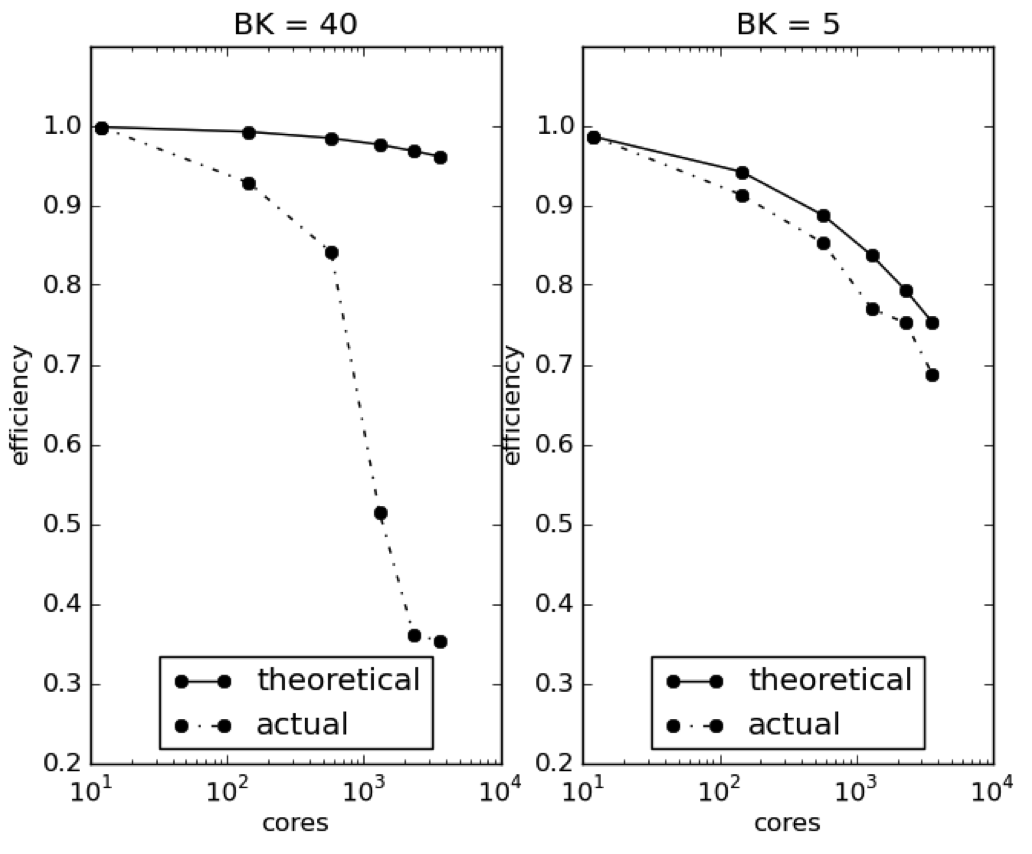
\includegraphics [width=.85\textwidth, height=0.5\textheight ] {JagBlockStudy}
  \end{center}
  \caption{Modified Kobayashi Benchmark Problem 1, Efficiency as a Function of Number of Cores}
  \label{fig:JagBlockStudy}
\end{figure}

A few important conclusions can be drawn from the curves in Figure~\ref{fig:JagBlockStudy}. One is that the increase in simultaneous work that should come from using smaller computational blocks is overwhelmed by communication latency in practice. When $B_{K}$ = 40 the theoretical efficiency remains high as the number of cores increases, but the measured efficiency becomes quite low: for 3,600 cores $\epsilon_{max}$ = 0.96 and $\epsilon$ = 0.35. It is expected that more blocks would be better, but when the number of cells/block becomes too small the cores spend more time waiting to pass data than doing useful work. 

Another relevant finding is that the theoretical and actual efficiencies match when there is a minimum block size. When larger computational spaces are used (smaller $B_{K}$) communication does not become a dominant factor. This restricts the extent of spatial decomposition by limiting the number of blocks used for a given spatial mesh. For a 500M cell problem, the limitation is 15,000 - 20,000 cores. 

Once a problem is spatially decomposed beyond the minimum block size limit, communication latency begins to dominate solution time and using more cores will be of little benefit. This is caused by the KBA algorithm. In order to take advantage of more cores for a given problem size, another area of phase space must be parallelized: energy, the remaining unparallelized dimension. 

It is worth noting that the phrase ``for a given problem size'' is important when stating that a problem cannot efficiently use more cores by being further decomposed in space alone. If a system is meshed more and more finely, then more cores can be used. For problems of interest today, however, using meshes large enough to use the full Jaguar machine efficiently necessitates meshing beyond discretizations of physical interest in nuclear engineering. 

One last point is that the current decomposition only allows for refining a problem in space and angle to increase parallelization and keep the wall time low as problems get larger. More finely resolving energy, which is desired for many of today's calculations, only makes the problem more expensive. No matter what mesh is used, KBA will never be able to use of more cores to get better energy resolution.

%--------------------------------------------------------------------------------
%--------------------------------------------------------------------------------
\section{Background}
To understand the new method and why it enhances Denovo's performance, this section contains an explanation of scattering, an overview of relevant basic solvers, and information about how scattering is treated in the transport equation. The remainder of this chapter will primarily focus on the solution of $\ve{A}x = b$, where $\ve{A}$ is $n \times n$  and the exact form of $\ve{A}$ and $b$ will be specified in subsequent sections.

%--------------------------------------------------------------------------------
\subsection{Scattering}
One of the important contributions of this work is the implementation of a new mathematical approach for upscattering in transport calculations. When neutrons scatter, several outcomes with regard to energy are possible. One outcome is that neutrons can stay within their energy group, called within-group scattering, and is described by the $[\ve{S}]_{gg}$ portion of the scattering matrix. Neutrons can also move into a lower energy group, or downscatter, given by $[\ve{S}]_{gg'}$ where $g > g'$. In some cases neutrons can gain energy and upscatter, described by $[\ve{S}]_{gg'}$ where $g < g'$. 

Material cross sections can be highly energy dependent and therefore high-resolution data in certain energy ranges may be needed to accurately capture the physics of the system. Upscattering is often important in problems where detailed information about low-energy, or thermal, neutrons is needed. In light-water reactors, thermal neutrons cause the bulk of the fission so these are systems that often need cross sections with upscattering terms.  

As mentioned in Chapter \ref{sec:Chp1}, the transport problem is broken into outer iterations and inner iterations. The inner iterations correspond to the within-group equations. Each inner iteration converges the flux for just one group by solving a fixed source problem for that group. The fixed source contains the appropriate combination of inscattering from other groups, an external source, and a source from fission.  The outer iterations are over the entire set of energy groups: all of Equations \eqref{eq:group-equations}. If a problem does not have upscattering, the equations can be quickly solved using one outer iteration. 

%--------------------------------------------------------------------------------
\subsection{Solver Basics}
There are two categories of methods for solving $\ve{A}x = b$, direct and iterative. Direct methods solve the problem by inverting $\ve{A}$ and setting $x = \ve{A}^{-1}b$. If $\ve{A}$ is invertible this can be done explicitly. $\ve{A}$ is often not invertible, so most direct methods are based on factoring the coefficient matrix $\ve{A}$ into matrices that are easy to invert. The problem is then solved in pieces where each factored matrix is inverted to get the final solution. An example where this is done is LU factorization. These methods are often robust and require a predictable amount of time and storage resources. However, direct methods scale poorly with problem size, becoming increasingly expensive as problems grow large \cite{Benzi2002}.

Iterative methods compute a sequence of increasingly accurate approximations to the solution. They generally require less storage and take fewer operations than direct methods, though they may not be as reliable. Iterative methods are highly advantageous for large problems because direct methods become intractable for systems of the size of those of interest here. For this reason the nuclear energy industry tends to use iterative methods for transport calculations \cite{Birkhoff1984}, \cite{Benzi2002}. 

Within the category of iterative methods, two further subdivisions can be made that will be useful in this work. Some methods only place data from previous iterations on the right hand side of the equation. The order in which those equations are solved is then irrelevant because only the previous iterate is needed. The other class of methods place data from both the previous and current iteration on the right hand side. These methods are fundamentally sequential and must be solved in order. These two categories will be referred to as order independent and order dependent, respectively. 

\subsubsection{Richardson Iteration}
The simplest iteration scheme used by the nuclear community is source iteration (SI), also known as Richardson iteration. SI is applied to the within-group space-angle iterations. Some other method is needed to conduct outer iterations over energy. Richardson iteration can be thought of as a two-part process for the neutron transport equation, where $\bar{Q}$ includes all sources and $k$ is the inner iteration index:
%
\begin{align}
  \ve{L}[\psi]_g^{k+1} &= \ve{MS} [\phi]_g^k + [\bar{Q}]_{g} \:,   \label{eq:SIpsi} \\
  [\phi]_g^{k+1} &= \ve{D}[\psi]_g^{k+1} \:.
  \label{eq:SIphi}
\end{align}
%
The spectral radius determines the speed of convergence and is $c = \Macro_s / \Macro$. For problems dominated by scattering, SI will converge very slowly \cite{Evans2009d}. While this is the simplest iterative method used, there are other more sophisticated methods available. 

\subsubsection{Jacobi}
The Jacobi method is known as the method of simultaneous displacements \cite{LeVeque2007}. This could be applied as the outer iteration method over energy and can be written as follows where $j$ is the outer iteration index:
%
\begin{equation}
  \ve{L} [\psi]_{g}^{j+1} = [\ve{M}] [\ve{S}]_{gg}[\phi]_{g}^{j} +   [\ve{M}]\bigl(\sum_{g'=1}^{g-1} [\ve{S}]_{gg'}[\phi]_{g'}^{j} + \sum_{g'=g+1}^{G} [\ve{S}]_{gg'}[\phi]_{g'}^{j} + [q_{e}]_{g} \bigr) \label{eq:Jacobi} \:. 
\end{equation}
%
The Jacobi method is order independent since all terms on the right are at the old iteration level. Jacobi is unconditionally stable and linearly convergent, but may converge very slowly. The convergence of Jacobi is governed by its spectral radius \cite{LeVeque2007}. 

\subsubsection{Gauss Seidel}
Gauss Seidel (GS) is known as the method of successive displacements \cite{LeVeque2007}. It is commonly used as the outer iteration method over energy and can be written as follows:
%
\begin{equation}
  \ve{L} [\psi]_{g}^{j+1} = [\ve{M}] [\ve{S}]_{gg}[\phi]_{g}^{j+1} +   [\ve{M}]\bigl(\sum_{g'=1}^{g-1} [\ve{S}]_{gg'}[\phi]_{g'}^{j+1} + \sum_{g'=g+1}^{G} [\ve{S}]_{gg'}[\phi]_{g'}^{j} + [q_{e}]_{g} \bigr) \label{eq:GaussSeidel} \:. 
\end{equation}
%
The GS method is order dependent, containing terms on the right hand side at both the new and old iterates. Once the space-angle iterations for each upscattering group are completed for one outer iteration, the right hand side is recalculated and the within-group calculations are repeated. This goes on until the entire system converges \cite{Evans2009d}. 

Gauss Seidel is also unconditionally stable and linearly convergent, but may converge very slowly. The convergence of GS is also governed by its spectral radius, $\rho$, though it converges twice as fast as the Jacobi method \cite{LeVeque2007}. 

The spectral radius of Gauss Seidel has been found for various materials by solving the eigenvalue problem $(\ve{T} - \ve{S}_{D})^{-1}\ve{S}_{U} \xi = \rho \xi$, where $\ve{T}$ is the matrix of total cross sections, $\ve{S}_{U}$ is the upper triangular portion of $\ve{S}$, $\ve{S}_{D}$ contains the diagonal and lower triangular portion, and $\xi$ is the eigenvector. This eigenvalue problem comes from Fourier analysis. The spectral radii for some materials of practical interest determined using cross sections with 41 thermal upscattering groups are: graphite = 0.9984, heavy water = 0.9998, and iron = 0.6120 \cite{Adams2002}, \cite{Evans2009d}. Problems containing graphite or heavy water would converge very slowly if GS were used.   

\subsubsection{Krylov methods}
Krylov methods\footnote{For a detailed discussion of Krylov methods and how they work see Appendix \ref{sec:AppendixB}.} are a powerful class of subspace methods that can be ideal for solving various types of linear and eigenvalue problems. A Krylov method solves $\ve{A}x = b$ by building a solution from a Krylov subspace generated by an iteration vector $v_{1}$. At iteration $k$, the subspace is:
%
\begin{equation}
  \mathcal{K}_{k}(\ve{A},v_{1}) \equiv span\{v_{1}, \ve{A}v_{1}, \ve{A}^{2}v_{1}, ..., \ve{A}^{k-1}v_{1}\} \:.
  \label{eq:Krylov-subspace}
\end{equation}
%
The choice of $v_{1}$ varies, but $v_{1} = b$ is common. When the problem is presented as $\ve{A}z = r_{0}$ where $r_{0} \equiv b - \ve{A}x_{0}$ and the solution is $x_{k} = x_{0} + z$, then $v_{1} $ is often chosen to be $r_{0}$. Note that $x_{0}$ is the initial guess and $x_{k}$ is the solution approximation at step $k$  \cite{Ipsen1998}.

The dimension of a Krylov space is bounded by $n$ because Krylov methods will give the exact solution after $n$ iterations in the absence of roundoff error. Interestingly, this technically makes Krylov methods a hybrid of direct and iterative methods because an exact answer can be obtained in a predetermined number of steps. Krylov subspace methods are nevertheless generally classified as iterative methods \cite{Birkhoff1984}.

Krylov methods are particularly useful in a few pertinent cases. One is when $\ve{A}$ is very large because fewer operations are required than traditional inversion methods like Gaussian elimination. Another is when $\ve{A}$ is not explicitly formed because Krylov methods only need the action of $\ve{A}$. Finally, Krylov methods are ideal when $\ve{A}$ is sparse because the number of operations are low for each matrix-vector multiplication. For deterministic transport codes, $\ve{A}$ is typically quite large, fairly sparse, and only its action is needed. The action of $\ve{A}$ is implemented through the transport sweeps \cite{Lewis1993}, \cite{Ipsen1998}.  

In the last few decades Krylov methods have been used widely to solve problems with appropriate properties for several reasons. Krylov methods are robust; the existence and uniqueness of the solution can be established; typically far fewer than $n$ iterations are needed when they are used as iterative solvers; they can be preconditioned to significantly reduce time to solution; only matrix-vector products are required; explicit construction of intermediate residuals is not needed; and they have been found to be highly efficient in practice \cite{Ipsen1998}, \cite{Knoll2004}. 

There are, however, a few drawbacks. In some cases Krylov methods can be very slow to converge, causing large subspaces to be generated and thus becoming prohibitively expensive in terms of storage size and cost of computation. Some methods can be restarted after $m$ steps\footnote{For information about restarted Krylov methods see Appendix \ref{sec:AppendixB}.} to alleviate this problem, keeping the maximum subspace size below $\mathcal{K}_{m+1}$.  The relatively inexpensive restart techniques can reduce the storage requirements and computational costs associated with a slow-converging problem such that they are tractable. Preconditioners can also help by reducing the number of iterations needed. Development of appropriate preconditioners is an active area of research \cite{Warsa2004a}, \cite{Ipsen1998}, \cite{Knoll2004}. 

In the 1970s interest in Krylov methods in the wider computational community began to increase after it was demonstrated that these methods can converge quickly. At first Krylov methods were restricted to problems where $\ve{A}$ is symmetric positive definite (SPD). These are methods such as conjugate gradient (CG), MINRES, SYMMLQ, and others. Then, Krylov methods for non-symmetric matrices became a focus, including the Generalized Minimum Residual (GMRES) and BiConjugate Gradient Stabilized (BiCGSTAB) methods \cite{Barrett1994}, \cite{Benzi2002}. The transport problem has characteristics that make it well suited for solution with Krylov methods, and these methods are used in several novel ways throughout this work.

%--------------------------------------------------------------------------------
\subsection{Current Scattering Solution Methods}
Three of the four methods just discussed are used in many transport codes, including Denovo. The inner iterations are done with either SI or a Krylov method and the outer iterations are done with Gauss Seidel. In this chapter the energy block consists of the upscattering block. The operator notation developed in Chapter~\ref{sec:Chp1} is used throughout the balance of this work. The fixed source problem will be presented here, but the discussion can be easily extended to eigenvalue calculations by using the fission source for each group in place of the external source. 

A simple five group example matrix will be used for reference throughout this subsection and subsection~\ref{subsec:KrylovMethod}. The matrix illustrates the structure of $\ve{S}$  when groups 1 and 2 have only downscattering and the upscatter block is defined over the range [$g_{1}$ = 3, $g_{2}$ = 5]:
%
\begin{equation}
  \mathbf{S}  =     \begin{pmatrix}
      [\ve{S}]_{11} &0 & 0 & 0 & 0 \\
      [\ve{S}]_{21} & [\ve{S}]_{22} & 0 & 0 & 0 \\
      [\ve{S}]_{31} & [\ve{S}]_{32} & [\ve{S}]_{33} & [\ve{S}]_{34} & [\ve{S}]_{35} \\
      [\ve{S}]_{41} & [\ve{S}]_{42} & [\ve{S}]_{43} & [\ve{S}]_{44} & [\ve{S}]_{45} \\
      [\ve{S}]_{51} & [\ve{S}]_{52} & [\ve{S}]_{53} & [\ve{S}]_{54} & [\ve{S}]_{55}
    \end{pmatrix} \:.
    \label{eq:exmp-matrix}
\end{equation}

\subsubsection{Downscattering}
Groups that only contain downscattering can be solved using forward substitution. The within-group transport equations are the same as in Equation \eqref{eq:GaussSeidel}, but the upscattering term goes away. The equation is combined with Equation \eqref{eq:SIphi} and rearranged to eliminate $[\psi]_{g}$ such that the unknown quantity is $[\phi]_{g}$. 

Each group equation is solved sequentially starting with group $1$, so all group moments on the right hand side have already converged for the $j+1$ outer iterate. To help clarify notation, the moments being iterated upon will be designated $\phi^{*}$, the moments which are known at the $j+1$ iterate will be $\phi^{new}$ and those from $j$ will be $\phi^{old}$. Together this looks like:
\begin{align}
  &[\phi]_{g}^{*} =  \ve{DL^{-1}}[\ve{M}][\ve{S}]_{gg}[\phi]_{g}^{*} +  \ve{DL^{-1}}[\ve{M}] \bigl(  \sum_{g'=1}^{g-1} [\ve{S}]_{gg'}[\phi]_{g'}^{new} + [q_{e}]_{g} \bigr) \label{eq:within-unarranged} \:;  \\
  %
  &\underbrace{\bigl( \ve{I} - \ve{DL^{-1}}[\ve{M}][\ve{S}]_{gg} \bigr)}_{\tilde{\ve{A}}}[\phi]_{g}^{*} = \underbrace{\ve{DL^{-1}}  [\ve{M}] \bigl(  \sum_{g'=1}^{g-1} [\ve{S}]_{gg'}[\phi]_{g'}^{new} + [q_{e}]_{g} \bigr) }_{\tilde{b}} \label{eq:within-krylov} \:. 
\end{align}
%
For example matrix \eqref{eq:exmp-matrix}, the first and second groups would be solved using this strategy. That means forward substitution would be used to solve this part of the scattering matrix:
%
\begin{equation}
  \mathbf{S_{down}} = \begin{pmatrix}
      [\ve{S}]_{11} &0 & 0 & 0 & 0 \\
      [\ve{S}]_{21} & [\ve{S}]_{22} & 0 & 0 & 0 \\  
      \end{pmatrix} \:.
          \label{eq:down-matrix}
\end{equation}
%
For group 2, Equation~\eqref{eq:within-krylov} would be:
%
\begin{equation}
  \bigl( \ve{I} - \ve{DL^{-1}}[\ve{M}][\ve{S}]_{22} \bigr)[\phi]_{2}^{*} = \ve{DL^{-1}}[\ve{M}] \bigl( [\ve{S}]_{21}[\phi]_{1}^{new}  + [q_{e}]_{1} \bigr) \:.
\end{equation}

Once the equations have been arranged in this way, a within-group solver is used to find the $j+1$ value for $[\phi]_{g}$. This iterative method could be source iteration, a Krylov method, or some other choice. When using a Krylov solver, the first step is always to calculate $\tilde{b}$. 

In Denovo, Aztec \cite{Heroux2007} provides the linear within-group solver. The Aztec solver is given an operator that implements the action of $\tilde{\ve{A}}$, the right hand side $\tilde{b}$, and an iteration/solution vector $v$. The action of $\tilde{\ve{A}}$ is implemented by doing the following for a group $g$:
\begin{enumerate}
  \item matrix-vector multiply: $y_{g} = [\ve{M}][\ve{S}]_{gg} v_{g}$,
  \item sweep: $z_{g} = \ve{DL}^{-1} y_{g}$,
  \item return: $v_{g} \leftarrow v_{g} - z_{g}$.
\end{enumerate}
In this implementation the Aztec solver iterates on $v_{g}$, which represents $[\phi]_{g}$, until it is converged for that group. Once the updated moments are returned, the next group is iterated upon. 

An iterative solver is used for even these simple forward substitution calculations because $\tilde{\ve{A}}$ is never explicitly formed and thus Equation \eqref{eq:within-krylov} cannot be solved directly. Only one outer iteration is required in fixed source problems when there is no upscattering because once each group is converged it is not changed by lower energy groups. 

%Another way to look at this is that the right hand side of the equation is not changed by subsequent iterations, so solving $[\tilde{\ve{A}}]_{g} [\phi]_{g} = [\tilde{b}]_{g}$ will give the same answer both before and after all subsequent downscattering moments, $[\phi]_{g'}, g' \ne g$, are determined. 

\subsubsection{Upscattering}
When upscattering is present, the lower energy groups do influence the higher energy groups so multiple outer iterations are needed. The within-group equations for groups $[g_{1}, g_{2}]$ now contain contributions from both higher and lower energy groups. 

The Gauss-Seidel (GS) method is commonly used to handle the upscattering block and, using the same notation as with downscattering, can be written as follows:
%
\begin{equation}
\underbrace{\bigl( \ve{I} - \ve{DL^{-1}}[\ve{M}][\ve{S}]_{gg} \bigr)}_{\tilde{\ve{A}}} [\phi]^{*}_{g} = \underbrace{\ve{DL^{-1}}[\ve{M}] \bigl( \sum_{g'=1}^{g-1}[\ve{S}]_{gg'}[\phi]^{new}_{g'} + \sum_{g'=g+1}^{g2} [\ve{S}]_{gg'}[\phi]^{old}_{g'}  + [q_{e}]_{g} \bigr)}_{\tilde{b}}  \:.
 \label{eq:up-GS}
\end{equation}
%
Because lower energy groups that have not been solved yet contribute neutrons to higher energy groups that have already been solved, the upscatter block becomes its own iteration loop. The solution procedure is exactly the same as with downscattering only, except that once the $[\phi]_{g_{1}}$ to $[\phi]_{g_{2}}$ moments are converged $\tilde{b}$ is recalculated and the outer iterations over the upscatter block are repeated. Most deterministic transport codes use GS for upscattering. Because GS is order dependent in energy, decomposition in energy is not possible \cite{Evans2009d}. 

%-----------------------------------------------------------
%-----------------------------------------------------------
\section{Past Work}
Now that the basics of inner and outer iterations have been described, past solution methods can be understood. 

\subsection{Inner Iterations}
Source iteration was historically the inner iteration method of choice. SI is still often used, but now it is typically accelerated to improve convergence. Unfortunately, even accelerated SI is not always fast or robust enough for new calculations of interest. The slow convergence of SI is part of what motivated interest in Krylov methods. 

In 1977 CG, which requires $\ve{A}$ to be symmetric positive definite (SPD), was used in solving the transport equation for the first time \cite{Lewis1977}. $\ve{A}$ is only SPD for the discretized transport equation when a symmetric quadrature set is used for the \Sn approximation and the scattering is isotropic. Otherwise, the matrix is non-symmetric. 

GMRES, which works for non-symmetric systems, was applied in a transport problem with anisotropic scattering for the first time in 1991 \cite{Adams2002}. It was not until Krylov methods for non-symmetric matrices were developed, restart methods became well known, and computer architecture could accommodate the storage required by Krylov subspaces needed in transport problems that the nuclear community began more widely using Krylov methods. 

With a few exceptions, Krylov methods have only been applied in neutron transport to the inner iterations. In some cases Krylov methods have been used as stand-alone iterative schemes to perform the within-group solves. In other cases they have been used as one part of the inner iteration process. For example, diffusion or transport synthetic acceleration (D/TSA) is often chosen to precondition SI as the inner iteration solver, where CG is used to solve the D/TSA portion of the calculation \cite{Gupta2004}. Krylov methods have also been applied to the diffusion equation when a few groups have been used \cite{Suetomi1988}, \cite{Verdu1999}.

Krylov methods have so far been largely restricted to inner iterations or few-group diffusion problems primarily because of hardware limitations and momentum of existing code structure. A Krylov subspace of size 30 can use a lot of memory when $v$ holds many variables. Until very recently, computers were not large enough to handle subspace iteration methods for a 3-D, anisotropic transport problem with many energy groups.  

Further, the inner-outer iteration structure has been successfully used in computational neutronics for quite some time, and it can take substantial effort to modify the fundamental solution processes in large codes. Often there is a time lag between when new methods are developed and when they find wide-spread incorporation, adding to the delay in implementing new methods in existing codes.

\subsection{Outer Iterations}
When upscattering is present, Gauss Seidel is almost universally used as the outer iteration solver. As noted above, GS can converge very slowly for some systems containing materials like heavy water, which are of interest to the nuclear community. Such slow convergence is part of the motivation for this work, which develops a method to replace GS for the upscatter block. 

There is one case where a Krylov method was used in a fixed source problem for something besides within-group solves. In 2004 Warsa et.\ al.\ used restarted flexible GMRES (FGMRES(m)) as an intermediate-level iteration over upscatter groups (what this chapter calls the outer iterations). In one upscattering case they used a Krylov solver for within-group iterations, FGMRES(m) over the upscatter block, and an implicitly restarted Arnoldi method for the eigenvalue outer iteration. They compared this to using block GS for the upscatter intermediate-level iteration. They found that using a Krylov solver rather than block Gauss Seidel for upscatter was faster. This was the only work identified that used a Krylov method for upscattering \cite{Warsa2004a}. 

Choosing to use an intermediate-level Krylov solver while still doing inner iterations with a Krylov solver is a bit of a strange choice. This choice was probably motivated by the desire to minimize changes to the code. By keeping the traditional inner-outer iteration method and adding a Krylov layer in between, very little code modification was needed. 

The methods that have been used in the past dictate an inner-outer iteration structure and limit parallelization to space and angle. No transport codes were found that have been parallelized in energy nor that deal with upscattering in a way different from what has been explained above. 

%-----------------------------------------------------
%----------------------------------------------------- 
\section{Multigroup Krylov Solver}
Section \ref{sec:DenAndPar} demonstrated that Denovo is limited in the number of cores it can use effectively. In addition to enhanced parallelism, there is also a need for faster solution algorithms for all parts of the code so Denovo can be used to solve very large systems. To address these issues, a new solver was implemented that applies a Krylov method to an entire block of energy groups rather than to only one group at a time. This replaces the inner-outer iteration structure with just one level of iteration because all groups can be converged simultaneously. 

\subsection{Method}
\label{subsec:KrylovMethod}
The first goal of this project is to decompose the upscatter block in energy so that portion of phase space can be parallelized. This goal can be achieved in a straightforward way by solving the entire upscattering block as one entity with a Krylov method rather than solving one group at a time. 

In the new method there are two ways to partition the energy groups: over all groups and over upscattering groups only \cite{Evans2010}. Partitioning over upscattering groups only is more complex, so will be described in greater detail here. In this case, the downscatter groups are treated the same way as before. For the example case, $[\phi]_{1}$ and $[\phi]_{2}$ are solved in the downscattering only calculations and are known by the time the upscatter block is reached. The portion of the scattering matrix shown in Equation \eqref{eq:up-source-matrix}, operates on these moments. 
%
 \begin{equation}
  \mathbf{S_{up\_source}}  =     \begin{pmatrix}
      [\ve{S}]_{31} & [\ve{S}]_{32}  \\
      [\ve{S}]_{41} & [\ve{S}]_{42}  \\
      [\ve{S}]_{51} & [\ve{S}]_{52} 
    \end{pmatrix} 
    \label{eq:up-source-matrix} 
 \end{equation}
%
The remainder of the scattering matrix, shown in Equation \eqref{eq:up-matrix}, operates on $[\phi]_{3-5}$. The idea behind the new solver is to treat $[\phi]_{3-5}$ as one vector to be solved at one time, rather than three vectors to be solved in series. 
%
 \begin{equation}
  \mathbf{S_{up\_block}}  =     \begin{pmatrix}
      [\ve{S}]_{33} & [\ve{S}]_{34} & [\ve{S}]_{35} \\
      [\ve{S}]_{43} & [\ve{S}]_{44} & [\ve{S}]_{45} \\
      [\ve{S}]_{53} & [\ve{S}]_{54} & [\ve{S}]_{55}
    \end{pmatrix} 
    \label{eq:up-matrix}
\end{equation}

Instead of $\tilde{G} = g_{2 }- g_{1}$ separate within-group upscattering equations, the new method has \emph{one} block upscattering equation. To do this, Equation \eqref{eq:up-GS} is modified to apply to a block instead of a series of groups. The entire upscatter block, or matrix \eqref{eq:up-matrix}, moves to the left because it acts on the upscattering-block-vector being iterated upon ($[\phi]_{3-5} = \phi^{*}$). The upscatter source, $\ve{S}_{\text{up\_source}}$ of matrix \eqref{eq:up-source-matrix}, remains on the right because it is only acting on the downscattering groups that have been solved at the current iteration level ($[\phi]_{1-2} = \phi^{new}$). The form of the new strategy is shown in Equation \eqref{eq:up-krylov} and looks very much like Equation \eqref{eq:within-krylov}.
%
\begin{equation}
 \underbrace{ \bigl( \ve{I} - \ve{DL^{-1}}\ve{M}\ve{S}_{\text{up\_block}} \bigr)}_{\tilde{\ve{A}}} \phi^{*} = \underbrace{ \ve{DL^{-1}}\ve{M} \bigl( \ve{S}_{\text{up\_source}}\phi^{new} + q_{e} \bigr)}_{\tilde{\ve{b}}}  \label{eq:up-krylov} \\
\end{equation}

Applying the Krylov solver to this system is very similar to what was done before, but now the action of $\ve{\tilde{A}}$, or the matrix-vector multiply, is applied to the entire block at once instead of just one group:
%
\begin{enumerate}
  \item matrix-vector multiply: $y = \ve{M}\ve{S}_{\text{up\_block}} v$,
  \item sweep: $z = \ve{DL}^{-1} y$,
  \item return: $v \leftarrow v - z$.
\end{enumerate}
%
All that has happened to allow for solving the entire block at once is the redefinition of the iteration vector. This rearrangement makes the problem energy order independent. 

When partitioning over all groups, the downscattering groups are also included in the iteration vector. The entire scattering matrix is moved to the left and only the external or fission source is on the right. This works in the same way as when partitioning over upscattering, the iteration vector is simply larger.

This new formulation allows for parallelization of a block of groups in energy. The matrix vector multiply can be done at the same time for all groups in the block for each iteration. To see how this works over the upscattering block, refer to Figure \ref{fig:KrylovMultiply}. Each color can do its part of the matrix vector multiply at the same time as the other colors. After the separate multiplies, there is a global reduction so that every color has the updated $s$, or the same brown box. The rest of the application of A is straightforward and does not require any inter-color communication \cite{Evans2010}.
%
\begin{figure}[!h]
  \begin{center}
    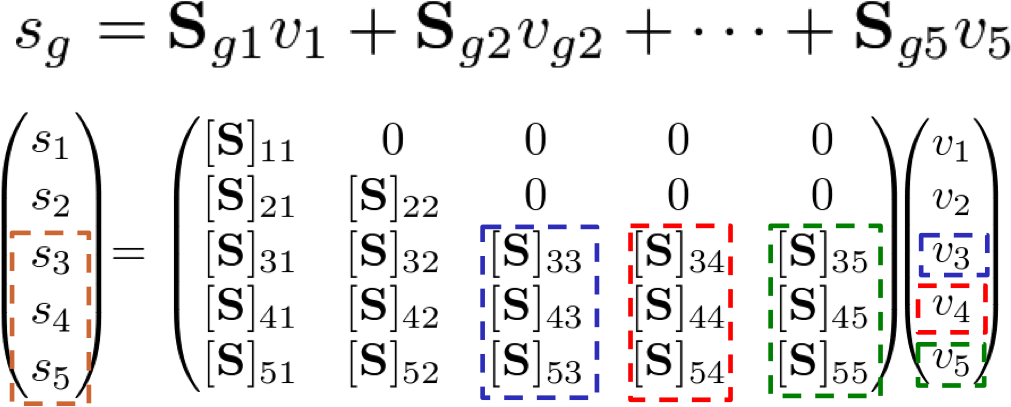
\includegraphics [width=.6\textwidth, height=0.2\textheight ] {KrylovGroupMultiply}
  \end{center}
  \caption{Parallel Implementation of Upscattering Matrix-Vector Multiply}
  \label{fig:KrylovMultiply}
\end{figure}

To implement the energy parallelization, the problem is divided into energy sets, with groups distributed evenly among sets. After each set performs its part of the matrix-vector multiply, a global reduce plus scatter is the only required inter-set communication. Since each set solves the entire spatial mesh with the same spatial decomposition, the established performance of spatial scaling does not change. A picture of the decomposition can be seen in Figure \ref{fig:EnergyDecomp}.
%
\begin{figure}[!h]
  \begin{center}
    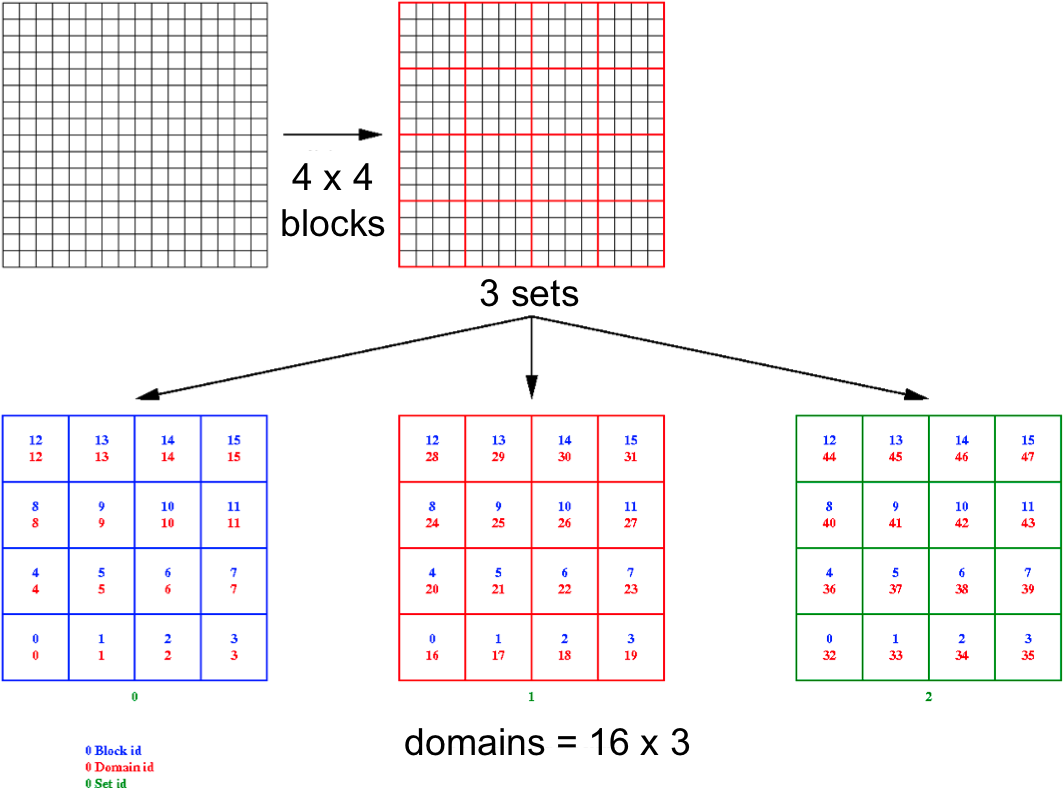
\includegraphics [width=.8\textwidth, height=0.45\textheight ] {EnergySets}
  \end{center}
  \caption{Energy Set Decomposition Added to Denovo \cite{Evans2011}}
  \label{fig:EnergyDecomp}
\end{figure}

It was demonstrated in Section \ref{sec:DenAndPar} that KBA becomes latency dominated when block size becomes small, limiting the number of cores that can be used for a given problem. Energy decomposition offers the ability to further decompose a problem, even after the practical limit of spatial performance for a given mesh has been reached, because scaling can be done across energy instead of space-angle. 

The number of cores is determined by the number of domains. Previously, the number of domains was equal to the number of spatial blocks. Now it is the product of number of energy sets and the number of spatial blocks. For example, with 10,000 spatial blocks (which KBA can handle) and 10 energy sets, Denovo can use 100,000 cores \cite{Evans2011}, \cite{Evans2010}. KBA would not be able to efficiently use 100,000 spatial blocks for meshes of practical interest. This dramatically increases the scalability of Denovo.

Another benefit is having the option to scale in energy rather than space. Once the desired mesh resolution and corresponding spatial decomposition is determined, using finer resolution in energy without energy parallelization makes the problem more costly in terms of both time and memory. To obtain more detailed flux data, fine-grained energy groups are needed. The energy decomposition capability makes this affordable. 

Before this work, no one had decomposed the transport equation in energy nor used one iteration level instead of two. This can now be done because there are machines large enough to store Krylov subspaces made from multiple group-sized iteration vectors, and these computers are large enough to warrant parallelization in energy. 

Note that the Jacobi method could have been used to decompose energy groups before because it is order independent in energy and does not have the large memory footprint associated with Krylov methods. However, there was no need to scale to so many cores and so there was no motivation for this development. Now that the scaling need exists, there is sufficient memory for Krylov methods. Krylov methods are the clear choice because they often converge faster than Jacobi \cite{LeVeque2007}. 

%--------------------------------------------------------------------------------
\subsection{Results}
The new method, which will be referred to as multigroup (MG) Krylov or block Krylov, has been implemented in Denovo. A few test problems were used to investigate the benefits of the new method. One was a small problem intended for initial scoping, and another was a full scale reactor calculation intended for more detailed study. Energy decomposition was investigated from the standpoint of both strong and weak scaling. The problems were also run without energy decomposition, i.e.\ using one energy set, to compare using Krylov instead of GS for the upscatter groups. First MG Krylov and GS are compared, then strong scaling studies are shown, and finally weak scaling is discussed.

\subsubsection{Gauss Seidel vs. Block Krylov}
The small problem was used first to compare GS to MG Krylov for multigroup upscattering. This is a cube of half iron and half graphite discretized with a 50 $\times$ 50 $\times$ 50 orthogonal mesh and decomposed into two spatial domains to use two cores. It is a 27-group problem with 13 upscattering groups and vacuum boundary conditions. An isotropic source is assigned everywhere to all energy groups, and the problem used $P_0$ and $S_4$. The iron plus graphite material composition was chosen for several reasons. Both materials are commonly found in nuclear reactors, graphite is highly scattering and creates a system with a large spectral radius for GS, and the cross sections were available with multiple upscattering groups.

The calculation took $3.51 \times 10^{3}$ seconds using MG Krylov, and the upscattering block converged in 43 GMRES iterations. With GS, the calculation took $2.87 \times 10^{4}$ seconds, or 718\% longer. This case converged in 44 Gauss Seidel iterations, each of which took about 124 GMRES inner iterations, or $\sim$5455 GMRES iterations all together. Note that the Krylov iterations in MG Krylov needed a subspace with a length dimension of 13 energy groups while the Krylov iterations in GS had a length of 1 energy group. This means the cost of the GMRES applications is not the same between solvers. Despite this, GS was very clearly more costly.

A version of this problem with a 10 $\times$ 10 $\times$ 10 grid and an $S_{8}$ angle set was also done. This compared GS, GS accelerated with a two-grid preconditioner (TTG; details are given in Section~\ref{sec:TTG}), and MG Krylov. The solver comparisons can be seen in Table~\ref{table:FeC GS Krylov}. ``GS Iters'' is the number of GS outer iterations and ``Krylov'' is the total number of Krylov iterations needed in the problem. This problem had no spatial or energy decomposition. The MG Krylov solver was faster than both accelerated and unaccelerated GS, and took far fewer Krylov iterations. 
%
\begin{table}[!h]
\caption{Iron Graphite Fixed Source Cube, Multigroup Krylov Compared to Gauss Seidel}
\begin{center}
\begin{tabular}{| l | c | l | c |}
\hline
Solver & GS Iters & Krylov & Time (s)\\[0.5ex]
\hline
GS &  12 & 1,727 & $1.12 \times 10^{2}$ \\
GS TTG & 11 & 1,687 & $1.99 \times 10^{2}$  \\
MG Krylov & n/a & 30 & $8.78 \times 10^{1}$ \\
\hline
\end{tabular}
\end{center}
\label{table:FeC GS Krylov}
\end{table}

Next a more realistic problem, the full-facility PWR core from the Section \ref{sec:DenAndPar}'s weak scaling study, was tested by Evans on the Jaguar machine. This PWR has 289 17 $\times$ 17 assemblies (157 fuel, 132 reflector) and vacuum boundary conditions. There are low, medium, and high enrichment fuel pins. A 2 $\times$ 2 spatial discretization per homogenized fuel pin was used giving 233,858,800 cells. $S_{12}$ was selected as the angular discretization. Two energy groups were used for this test to keep the total problem size small. To get a sense of the problem size, there were 78,576,556,800 unknowns.

It should be noted that Jaguar requires decompositions to be done in a certain way, which determines the number of domains that can be used. For example, keeping the spatial domain size exactly same when changing the number of energy sets is typically not possible so the closest available approximation is chosen instead.

\begin{table}[!h]
\caption{PWR900 with 2 groups, Multigroup Krylov Compared to Gauss Seidel}
\begin{center}
\begin{tabular}{| l | c | c | c | c |}
\hline
Solvers & Blocks & Sets & Domains & Solver Time (m) \\[0.5ex]
\hline
PI + TTG GS & 17,424 & 1 & 17,242 & 11.00 \\
PI + MG Krylov & 10,200 & 2 & 20,400 & 3.03 \\
\hline
\end{tabular}
\end{center}
\label{table:MGkrylovPWR}
\end{table}
%
Table~\ref{table:MGkrylovPWR} shows the results for the PWR900 problem. The goal was to compare MG Krylov and GS using the same number of domains, which required a different spatial decomposition. Power iteration (described in Chapter~\ref{sec:Chp3}) was used as the eigenvalue solver in both cases; GS again used GMRES for the inner iterations and GS was accelerated with TTG. While GS had 15.5\% fewer domains than MG Krylov, it took 263\% longer. Clearly the MG Krylov method was faster than GS for this problem, even when GS was preconditioned and MG Krylov was not. 

In both test cases the new Krylov multigroup solver significantly outperformed Gauss Seidel. The Krylov method took much less time and many fewer iterations, even when Gauss Seidel was accelerated. This demonstrates that the new multigroup solver provides substantial convergence improvement with only space-angle parallelization, which will help solve large and challenging problems. 

\subsubsection{Strong Scaling}
The first two test problems plus an additional system were used to examine strong scaling with energy sets. The iron graphite cube was used first, largely to verify multiset functionality rather than rigorously test scaling. The cube was expanded to a 100 $\times$ 100 $\times$ 100 mesh and decomposed into four spatial blocks to make it large enough to warrant using multisets. It should be noted that it is not expected that this problem will scale particularly well because it is still a small problem and the number of upscattering groups is prime. 

The number of energy sets was varied from 1 to 13. The test problems were run on the small orthanc cluster at ORNL.  The downscattering groups were solved with forward substitution as before, and the upscattering was solved with the Krylov multigroup solver. The upscattering groups converged in 104 GMRES iterations. Every calculation gave the correct flux.

\begin{figure}[!h]
  \begin{center}
    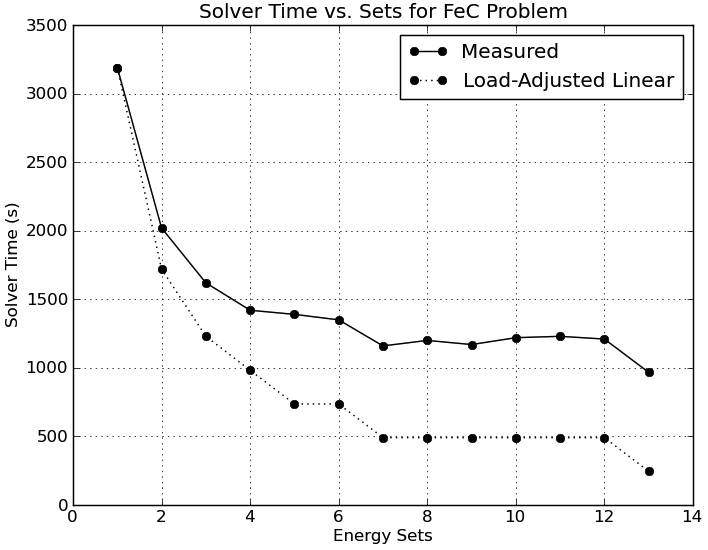
\includegraphics [width=.75\textwidth, height=0.45\textheight ] {FeCKrylovMultisets}
  \end{center}
  \caption{Iron Graphite Fixed Source Cube, Strong Scaling Study}
  \label{fig:FeGraphiteStudy}
\end{figure}
%
Figure~\ref{fig:FeGraphiteStudy} shows the measured time and the ``load-adjusted linear'' time. The perfect, i.e.\ linear scaling, solve time would usually be $(\frac{\text{base\_domains}}{\text{used\_domains}}) \times \text{base\_time}$. However, an alternative method was used to try to account for the load imbalance caused by the energy sets. There is no way to evenly divide 13 groups among energy sets, meaning at least one set always has one more group than the others. The sets with fewer groups must wait for the sets with more groups, which is not an efficient use of processing power. 

To account for the load imbalance, a factor was added that weights the time by the number of groups required for perfect energy load balance divided by the number of groups used. To get this, the maximum number of groups per set was determined, e.g.\ 13 groups / 2 sets = 7 groups. This was multiplied by the number of sets to get the number of groups needed for load balancing, e.g.\ 7 $\times$ 2 = 14. The base case used 4 cores and took $3.19 \times 10^{3}$ seconds. For 2 sets on 8 cores, $t_{\text{linear}} = \frac{4}{8}\times\frac{2\times7}{13} \times (3.19 \times 10^{3}) = 1.72 \times 10^{3}$.

The plotted results lead to a few conclusions. The actual time becomes increasingly different from the ideal time as the number of sets increases until about 5 sets, after which the perfect and measured time are different by an approximately constant amount. Using multisets had a good return on investment for a small number of sets. The efficiency, where efficiency is defined as the ideal time over the observed time, is about 85\% with 2 sets and goes down to about 53\% with 5 sets. Another way to say this is that with 5 sets a speedup of 4.33 would be ideal and a speedup of only 2.30 was observed. 

Overall, this test was not a very good scaling measure because of the load balancing issue. This is illustrated by the fact that the ideal time does not change between 7 sets using 28 cores and and 12 sets using 48 cores. A problem that is not expected to change calculation time when the number of cores increases by 70\% is not a good scaling test. However, this problem did demonstrate that the multiset implementation works, gets the correct answer, and may provide speedup where it makes sense.  

A 44 energy group cross section set was used with the PWR900 to study strong scaling in a more quantitative way than the iron and graphite cube. This many energy groups yielded \\ 1,728,684,249,900 degrees of freedom. Two spatial block - energy set combinations were used, detailed in Table~\ref{table:StrongCasesPWR}. Both cases used power iteration and the MG Krylov solver. Because of the decomposition restrictions, 9,024 spatial domains was the closest available approximation to 10,200.

Some general communication optimization was added to Denovo after these initial results were obtained and the two cases were redone. In Table ~\ref{table:StrongCasesPWR} ``Initial'' is the time taken by the solver before optimization and ``Optimized'' is the time afterwards. The optimization greatly improved the Base case results, reducing the solve time from 49.61 minutes to 38.33 minutes. Unfortunately, there was a negligible difference in the Study case's time. 
%
\begin{table}[!h]
\caption{PWR900 with 44 Groups, Strong Scaling Study}
\begin{center}
\begin{tabular}{| l | c | c | c | c | c |}
\hline
Case & Blocks & Sets & Domains & Initial (m) & Optimized (m) \\[0.5ex]
\hline
Base   & 10,200 & 11 & 112,200 & 49.61 & 38.33 \\
Study & 9,024    & 22 & 198,528 & 34.99 & 34.99 \\
\hline
\end{tabular}
\end{center}
\label{table:StrongCasesPWR}
\end{table}
%
Originally, the perfect time for the Study case was 28.04 minutes, giving an efficiency of 80\%. After optimization, the perfect scaling time became 21.66 minutes, reducing the scaling efficiency to 62\%. All of the data are plotted in Figure~\ref{fig:PWRstrongScaling}. 
\begin{figure}[!h]
  \begin{center}
    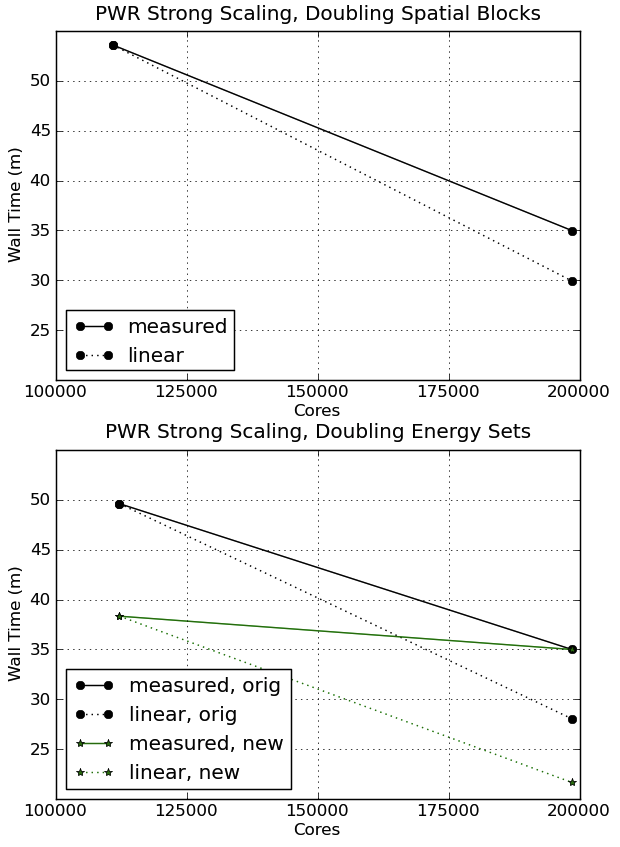
\includegraphics [width=.7\textwidth, height=.45\textheight ] {PWRstrongScaling}
  \end{center}
  \caption{PWR900 with 44 Groups, Strong Scaling Study}
  \label{fig:PWRstrongScaling}
\end{figure}

A variety of reasons have been identified for why the 200,000-core case did not improve as much as the 100,000-core case. Many of these are beyond the scope of this work: it is likely that the problem is not large enough to demonstrate strong scaling well; the block decomposition was not optimal; and there were communication collisions on the torus across the full machine that significantly slowed down communication \cite{Davidson2010}. 

Pertinent to this work, however, is that the multiset communication was not optimal. After each matrix-vector multiply a global reduction and scatter were done. In that process each block on every set got the contribution from every other set, and the data it scattered out was for all groups. The message size for all groups is large and can therefore be slow.

This communication pattern has since been improved by Evans and Davidson to a global reduction followed by a local scatter. When each space-energy domain communicates its updated flux after the multiply, it only communicates to the sets that need its contribution. If the upscattering on one set does not contribute to another set, there is no communication between those sets. The big change, however, is that the data scattered out is only the size of the groups on that set, not all groups \cite{Evans2011b}. In a 44 group problem with 22 sets, that changes the message size from 44-group length to 2-group length. This improvement has been implemented, but the PWR strong scaling calculations have not been repeated. 

To get an idea of the impact of the multiset reduction communication improvement, a fixed source 44 group problem was solved by Davidson with MG Krylov. Three different meshes and spatial decompositions were used for this problem, and each case used a variety of sets. The combinations can be seen in Table~\ref{table:MultisetCommOpt}.
%
\begin{table}[!h]
\caption{Test Cases for Multiset Communication Optimization Study}
\begin{center}
\begin{tabular}{| c | c | l |}
\hline
Mesh & Decomposition & Sets Used \\[0.5ex]
\hline
204 $\times$ 204 $\times$ 90 & 30 $\times$  60 $\times$  2 & 2, 4, 11, 22, 44 \\
408 $\times$ 408 $\times$ 90 & 60 $\times$  72 $\times$  2 & 1, 2, 4, 11, 44 \\
816 $\times$ 816 $\times$ 90 & 120 $\times$  144 $\times$  2 & 1, 2, 4, 11 \\
\hline
\end{tabular}
\end{center}
\label{table:MultisetCommOpt}
\end{table}

To measure the benefit of multiset communication optimization, the percentage of solve time spent doing the reduction across energy sets in the original ``Global Sum'' method is compared to the new ``Reduced Scatter'' method. The results for each mesh - set combination can be seen in Figure~\ref{fig:MultisetCommOpt}. The x-axis is number of energy sets and the y-axis is the percentage of solver time. For example, if the y-value is 3 that means 3\% of the time spent in the solver was used in multiset reduction communication. 
%
\begin{figure}[!h]
  \begin{center}
    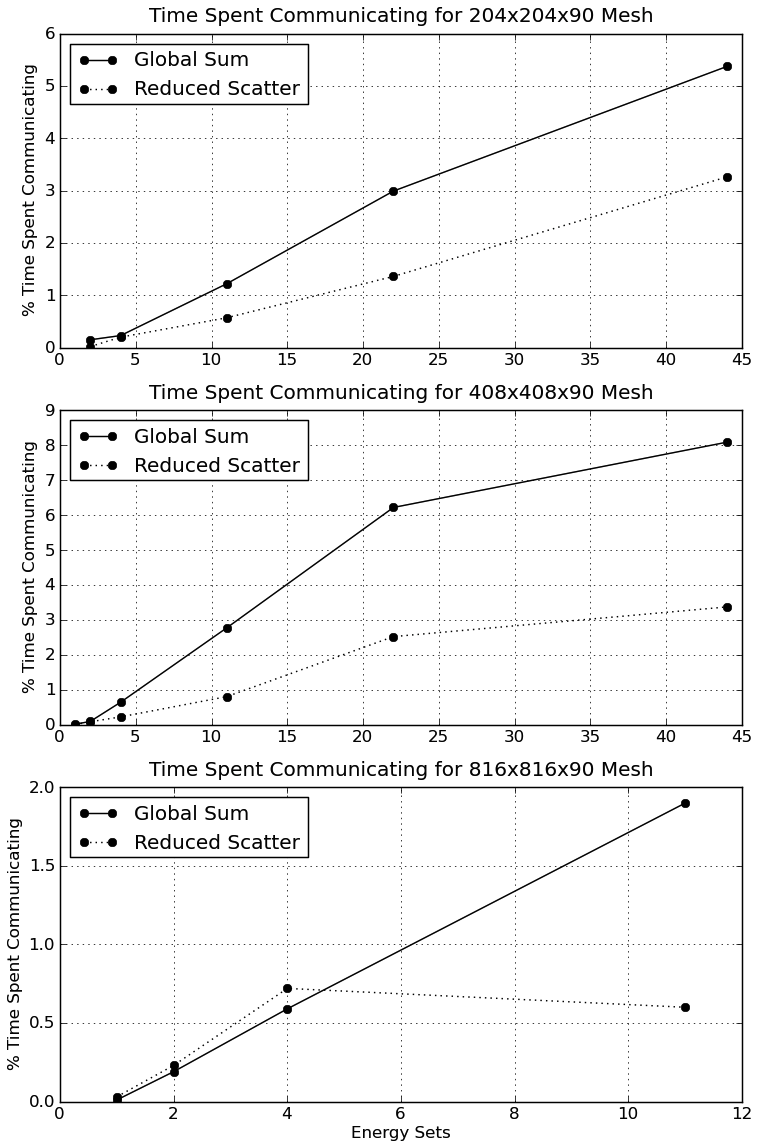
\includegraphics [width=.7\textwidth, height=0.85\textheight ] {MultisetCommOpt}
  \end{center}
  \caption{\% Time Used in Multiset Reduction Communication, Comparison of Old and New Strategies}
  \label{fig:MultisetCommOpt}
\end{figure}

These plots show that in nearly all cases the percentage of time spent on the reduction decreased. As the number of sets increases, the difference in percentage of time also increases. This makes sense because more sets require more reduction communication, so an improved method would have a bigger benefit. However, the spatial decomposition also plays a role since sets communicate across spatial boundaries. The benefit of the new strategy therefore differs for different spatial decompositions. In all cases though, the larger number of sets benefitted from the new implementation. 

These 44 group fixed source tests were also used to study strong scaling when both the general and multiset-specific communication optimizations were in place. These results, which can be seen in Figure~\ref{fig:FxdStrong}, are much better than both the iron graphite cube and PWR900 problems. 
%
\begin{figure}[!h]
  \begin{center}
    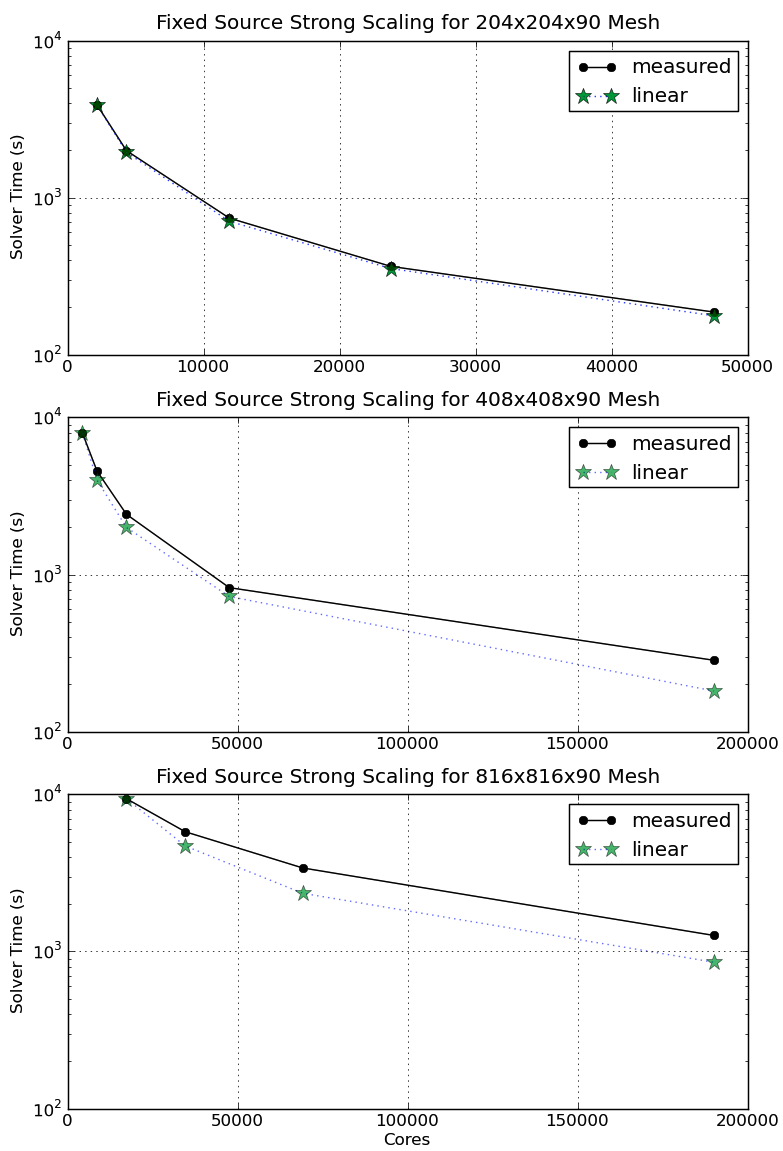
\includegraphics [width=.8\textwidth, height=0.95\textheight ] {FxdSrcKrylovStrongScaling}
  \end{center}
  \caption{Fixed Source Problem with 44 Groups, Strong Scaling Study}
  \label{fig:FxdStrong}
\end{figure}

The first mesh was only large enough for use on up to about 50,000 cores. The 2 set problem was used as the base case for computing linear time. The scaling on this problem was nearly perfect, with an efficiency of 95\% at 47,520 cores and 44 energy sets. 

The scaling was not as close to perfect with the two larger meshes, but it was still much better than the test cases without multiset communication optimization. The medium and large mesh versions both used 1 set as the base case. With the medium sized mesh the efficiency with 47,520 cores and 11 energy sets was 88\%, though the efficiency with 190,080 cores and 44 energy sets was only 64\%. Recall, however, that the PWR case compared 11 and 22 energy sets. If the 44 and 11 set cases are compared, the efficiency increases to 73\%.

The most energy sets used with the largest mesh version was 11. The efficiency with 11 sets on 190,080 cores compared to 1 set and 17,280 cores was 68\%. When comparing the 4 set case that used 69,120 cores to the 11 set case, the efficiency was 98\%, or nearly perfect. 

The 44 group fixed source problem showed that the block Krylov solver can scale fairly well in energy for a variety of spatial discretizations. While strong scaling in energy was not perfect for the medium and large meshes, it was far better than what could be obtained by scaling in space alone for even the largest mesh. The difference between the measured and linear times was not huge compared to the total solution time. 

Further, even when communication was not optimized the multigroup Krylov solver allowed Denovo to solve a real problem with over 1.7 trillion degrees of freedom in under 40 minutes. This problem would not have been practical to solve using the same 233M cell mesh without energy sets, relying on space-angle scaling alone. These results demonstrate that the block Krylov solver allows for the full use of leadership-class machines for problems where KBA would not.

\subsubsection{Weak Scaling}
Finally, the full-facility PWR problem was used for a weak scaling study. The two-group, 17,424-block, GS calculation (PI + TTG GS in Table~\ref{table:MGkrylovPWR}) was compared to the 44-group, 11-set, 10,200-block, MG Krylov calculation with the optimized general communication strategy, but without the multiset communication optimization. 

Recall that there were 78,576,556,800 unknowns when using 2 groups with 1 set on 17,424 cores, and 1,728,684,249,900 unknowns when using 44 groups with 11 sets on 112,200 cores. With weak scaling the problem size/core is typically kept constant. In these tests the problem size/core could not be held constant, so an adjustment factor was included. The number of energy groups were used to weight the problem size/core and that was used to get an adjusted solve time of 11.21 minutes for the MG Krylov calculation: $[(\frac{44}{2})(\frac{17,424}{112,200})]^{-1}\times38.33$ = 11.21. 

Efficiency for weak scaling is calculated by taking the ratio of the MG Krylov adjusted time to the reference time, or 11.21 over 11.00, giving an efficiency of 1.019. A plot of the weak scaling is shown in Figure~\ref{fig:PWRweakScaling}. Note that perfect weak scaling would maintain an efficiency of 1, thus the weak scaling observed here was very good. Recall that a weak scaling study using this same problem was reported in Section~\ref{sec:DenAndPar}. The performance with energy sets was markedly better than with KBA alone, showing that energy decomposition can improve weak scaling.
%
\begin{figure}[!h]
  \begin{center}
    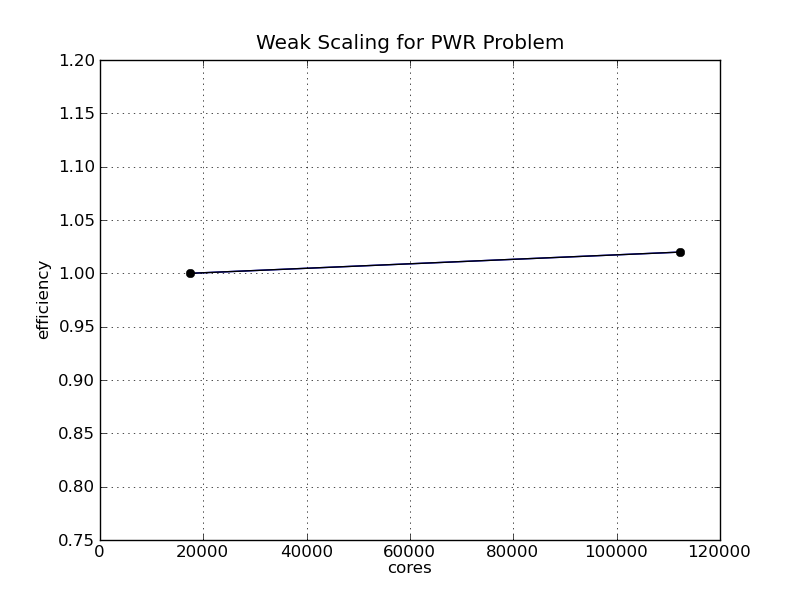
\includegraphics [width=.8\textwidth, height=0.48\textheight ] {PWRmyWeakScaling}
  \end{center}
  \caption{PWR900, Weak Scaling Study}
  \label{fig:PWRweakScaling}
\end{figure}

%-----------------------------------------------------
\subsection{Implications}
The tests just discussed show that the multigroup Krylov solver provides a time benefit both from using a Krylov solver for the equivalent of the outer iterations instead of Gauss Seidel and from the parallelization in energy that is enabled by this method. There were no deterministic transport codes found that decompose the upscatter calculation in energy, nor that only use one iteration level for the upscattering block. This decomposition is a new contribution to the field and helps alleviate the scaling limitations associated with KBA.   

There are a few reasons this has not been pursued before, primarily based on computer architecture and existing code capability. Memory has only become large enough to accommodate the necessary Krylov subspaces recently. Only in the last several years have there been computers with enough processing capability to allow for scaling to hundreds of thousands of cores, motivating energy decomposition. In addition, the inner-outer paradigm is at the core of most transport codes and in many cases it would take substantial effort to modify that structure. 

Note that an explicit block Jacobi method, which converges more slowly than GS by a factor of two, could have been used previously to decompose energy groups because it is explicit in energy and does not have the large memory footprint associated with Krylov methods. However, there was no need to scale to so many cores and so there was no motivation for this development. Now that the scaling need exists, there is sufficient memory for Krylov methods. Krylov methods are the clear choice because they often converge faster than Jacobi \cite{LeVeque2007}. 

Transport codes could have used machines with hundreds of thousands of cores without energy parallelization by solving problems with extremely large meshes. Doing this, though, would typically involve refining a problem's mesh for the sake of refining its mesh and not because the quality of solution requires more spatial resolution. In addition, this strategy does not address the need for increased energy resolution while decomposing in energy does. 

Overall, the tests showed the multigroup Krylov solver decisively accomplishes the goal of accelerating transport calculations by using new computers fully. The first two test problems illustrated that the block Krylov method does the multigroup iterations more quickly than the Gauss Seidel method. The strong scaling studies showed that the energy decomposition works and the method provides reasonably good strong scaling in energy. The weak scaling study showed that the MG Krylov method weak-scaled better than GS with only space-angle decomposition. 

\separatorpage{}
